\documentclass{llncs}
\usepackage{fullpage}

%load needed packages
\usepackage{graphicx}
\usepackage{array}
\usepackage{booktabs}
\usepackage[utf8]{inputenc}
\usepackage{amsmath} 
\usepackage{hyperref}


\begin{document}

\title{Task A}
\subtitle{Supervised Learning Model Evaluation Metrics}

\author{Diego De Pablo}
\institute{\email{depablodiego@uma.es} \\
Health Engineering. Málaga University.}

\maketitle 

\vspace{1cm} % Space down the title

\textit{
	This work investigates the performance of various classification methods in a supervised learning context, focusing on how certain techniques can yield misleadingly high metrics. Specifically, some methods that classify all samples into a single category may achieve better performance metrics compared to methods that accurately differentiate between positive and negative samples. The analysis highlights the importance of robust metrics like the Jaccard index and F-measure, which provide valuable insights into model performance. Ultimately, it underscores the necessity of understanding the specific goals of the analysis to determine which metrics are most relevant for evaluating a model’s effectiveness. }



\section{Introduction}

Artificial intelligence (AI) has emerged as a transformative solution to numerous challenges in a wide range of domains, often being viewed as a key to simple and efficient problem-solving. However, the performance of AI models must be critically assessed to understand their real-world applicability and limitations. In particular, supervised learning algorithms are often used in classification tasks, where the performance of these models can be evaluated through specific metrics.

In this work, we explore the key performance metrics derived from the \textit{confusion matrix} to assess and compare supervised learning models. These metrics include \textbf{Precision}, \textbf{Recall}, \textbf{Specificity}, \textbf{False Positive Rate}, \textbf{False Negative Rate}, \textbf{Accuracy}, \textbf{Spatial Accuracy}, \textbf{Jaccard Index}, and \textbf{F-measure}. These metrics are commonly used to provide a detailed view of a model’s performance across different dimensions. By understanding and comparing these metrics, we can gain insights into the strengths and weaknesses of the classification methods being evaluated.\cite{Liu2023}

In computational learning, applying classification algorithms to predict disease progression is critical for deriving meaningful insights from complex biomedical data. The primary focus of this project is to evaluate and compare the performance of several classification methods using a dataset relevant to disease classification. The analysis will focus on various aspects, including the dataset's class distribution, balance, and overall characteristics, and will use a range of well-established performance metrics.

The metrics used in this analysis provide a quantitative basis to assess each model’s strengths and limitations, allowing us to determine which algorithm performs best for predicting outcomes in the dataset. Specifically, we will implement an algorithm to calculate several well-known metrics based on the number of \textbf{True Positives (TP)}, \textbf{True Negatives (TN)}, \textbf{False Positives (FP)}, and \textbf{False Negatives (FN)}. 

These metrics will enable a comprehensive evaluation of each method's effectiveness in predicting for example disease progression. Furthermore, graphical representations, such as heatmaps and radar charts, will be used to provide a visual comparison of the methods. This will facilitate better understanding of each model's advantages and limitations, allowing for more informed decision-making when selecting the appropriate classification model.

\section{Dataset Description}

The aim of this work is to highlight the validation methods and explore examples ranging from realistic to exaggerated cases that, in certain scenarios, might be considered good results if certain metrics are ignored. Even though these results may seem favorable, they can actually be misleading. To demonstrate this, we will base our analysis on the following dataset (observe the figure \ref{fig:dataset}).

\begin{figure}[h!]
	\begin{center}  % Usamos el entorno 'center'
		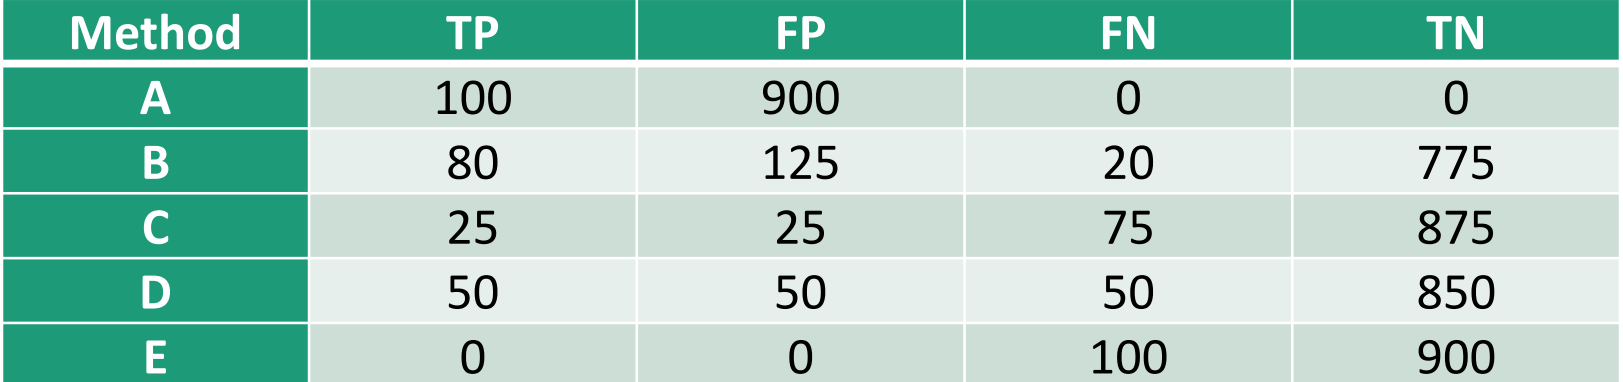
\includegraphics[width=1\textwidth]{images/dataset.png}
		\caption{The methods studied in this work}
		\label{fig:dataset}
	\end{center}
\end{figure}

\vspace{-20pt} % Ajusta este valor para reducir el espacio

The five hypothetical methods in this study are evaluated on a dataset of \textbf{1000 samples}, divided into \textbf{two classes} (positive or negative). This dataset is notably \textbf{imbalanced}, with 100 positive and 900 negative samples, which can lead to biased models and misleading metrics, as seen with methods A and E that perform poorly on specific measures.

Imbalanced datasets skew results, making some models appear more effective than they are. Techniques such as \textbf{oversampling}, \textbf{undersampling}, and \textbf{weight adjustment} are used to mitigate these effects, ensuring more reliable evaluations.

Figure \ref{fig:confusion} illustrates the percentage confusion matrix for each method, alongside a sixth matrix representing a perfect model that correctly identifies all positive and negative samples.



\begin{figure}[h!]
	\begin{center}  % Usamos el entorno 'center'
		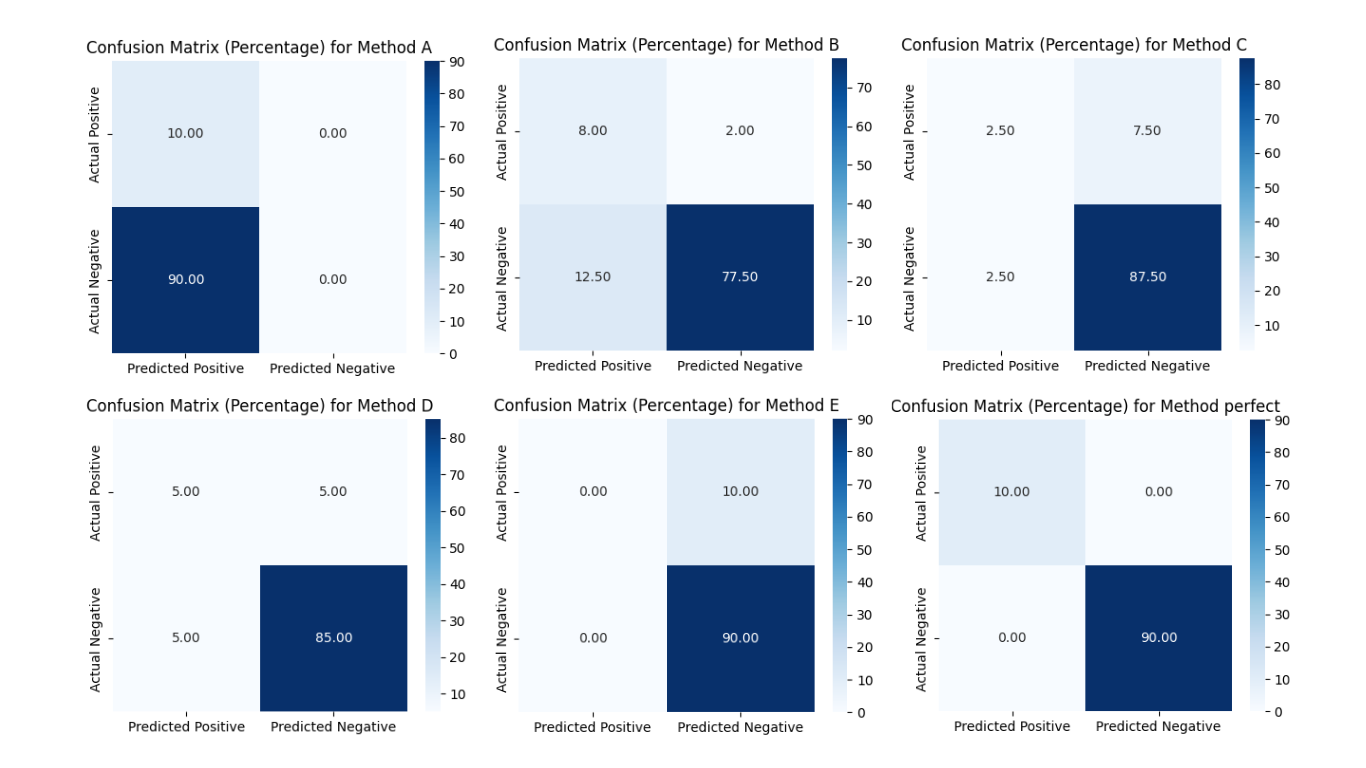
\includegraphics[width=1\textwidth]{images/5_metodos.png}
		\caption{6 confusion matrices, from A to E and the case of the perfect confusion matrix for this dataset}
		\label{fig:confusion}
	\end{center}
\end{figure}

Examining the confusion matrix for each method in relation to the ideal confusion matrix for the dataset reveals significant shortcomings in methods A and E, which classify all samples as either positive or negative. In contrast, methods B, C, and D demonstrate more realistic classification patterns, aligning more closely with the expectations of an effective machine learning approach. Although these methods approach the performance of a perfect model, they still exhibit a small percentage of false positives and false negatives. To determine which of these three methods is superior, it is essential to consider additional factors, such as validation metrics and the specific objectives for which the model is intended.

\section{Metrics Overview}

In this work, we implemented a function to compute various validation metrics using the true positives (TP), false positives (FP), true negatives (TN), and false negatives (FN) yielded by each method. The results are visualized in a heatmap  (see the Figure \ref{fig:heatmap}) to clearly present the performance of each method.

\begin{figure}[h!]
	\begin{center}  % Usamos el entorno 'center'
		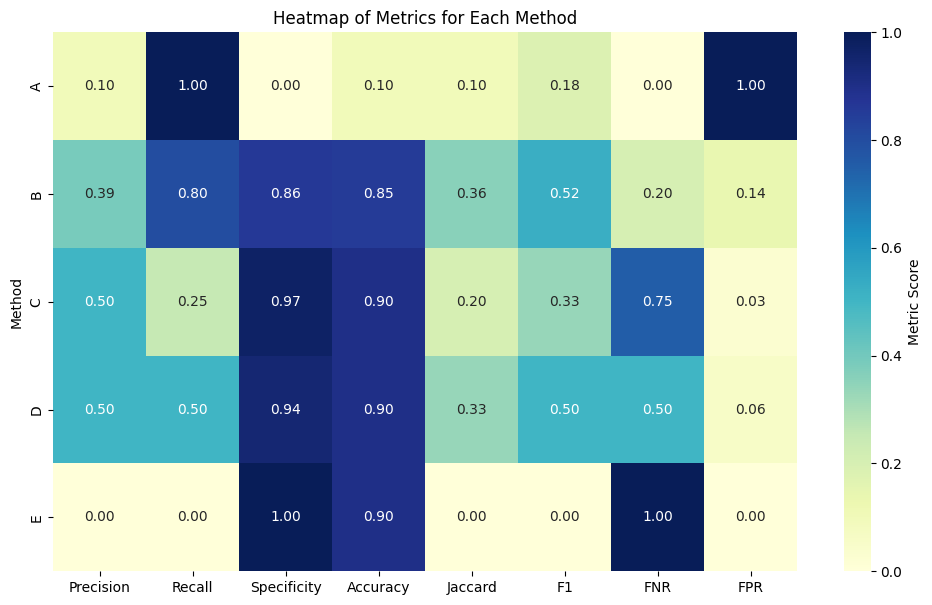
\includegraphics[width=1\textwidth]{images/heat_map.png}
		\caption{The methods studied in this work}
		\label{fig:heatmap}
	\end{center}
\end{figure}


\subsection{Summary of Expected Ranges}
\begin{itemize}
	\item Precision, Recall, Specificity, Accuracy, Jaccard, F1: Values range from 0 to 1, with higher values indicating better performance.
	\item FNR, FPR: Values range from 0 to 1, with lower values indicating better performance.
\end{itemize}


\subsection{Evaluation Metrics}

In machine learning, evaluation metrics are crucial for assessing model performance, particularly in classification tasks. Each metric provides unique insights into various aspects of the model's predictions. Below is a breakdown of the key metrics used in this study:

\subsubsection{Precision (PR)}
Also known as positive predictive value, measures the proportion of true positive predictions out of all positive predictions made by the model. It provides insight into the model's ability to avoid false positives.
\[
\text{Precision} = \frac{TP}{TP + FP}
\]
Indicates how many of the predicted positives were actually correct. It is especially useful when false positives are costly, such as in spam detection.

Looking at Table \ref*{tab:precision}, where each method is accompanied by its precision metric:
\begin{table}[h]
	\centering
	\begin{tabular}{|c|c|c|c|c|c|} 
		\hline 
		\textbf{Metric} & \textbf{A} & \textbf{B} & \textbf{C} & \textbf{D} & \textbf{E} \\ 
		\hline 
		\textbf{Precision} & 0.10 & 0.39 & \textbf{0.50} & \textbf{0.50} & 0.00 \\ 
		\hline 
	\end{tabular} 
	\caption{Precision metrics for each method.} 
	\label{tab:precision} 
\end{table} 
\vspace{-20pt}


It can be observed how methods C and D obtain the highest values, being 0.50 respectively, while the lowest is E with a precision of 0.00.

\subsubsection{Recall (RC)}
Also known as sensitivity or true positive rate (TPR), tells us how many of the actual positives were correctly identified by the model. It answers: "Out of all the real positive cases, how many were captured by the model?"

It is crucial in cases where missing a positive case is costly (false negatives are highly undesirable). In medical diagnoses, high recall means fewer missed cases of a disease.

\[
\text{Recall} = \frac{TP}{TP + FN}
\]

Looking at Table \ref{tab:recall}, where each method is accompanied by its recall metric:
\begin{table}[h]
	\centering
	\begin{tabular}{|c|c|c|c|c|c|} 
		\hline 
		\textbf{Metric} & \textbf{A} & \textbf{B} & \textbf{C} & \textbf{D} & \textbf{E} \\ 
		\hline 
		\textbf{Recall} & \textbf{1} & 0.80 & 0.25 & 0.50 & 0.00 \\ 
		\hline 
	\end{tabular} 
	\caption{Recall metrics for each method.} 
	\label{tab:recall} 
\end{table}

\vspace{-20pt}

Method A shows the highest recall, achieving a perfect score of 1 by capturing all positive cases. However, this metric does not consider negatives, and further analysis reveals that this method performs poorly overall. In contrast, Method E fails to identify any positives.

\subsubsection{Specificity (SP)} or true negative rate (TNR), measures the proportion of actual negatives that were correctly identified. It answers: "Of all the real negative cases, how many did the model correctly classify as negative?"

It is valuable when it's important to correctly identify negatives, such as in fraud detection, where you want to minimize false positives.

\[
\text{Specificity} = \frac{TN}{TN + FP}
\]

Looking at Table \ref{tab:specificity}, where each method is accompanied by its specificity metric:
\begin{table}[h]
	\centering
	\begin{tabular}{|c|c|c|c|c|c|} 
		\hline 
		\textbf{Metric} & \textbf{A} & \textbf{B} & \textbf{C} & \textbf{D} & \textbf{E} \\ 
		\hline 
		\textbf{Specificity} & 0.00 & 0.86 & 0.97 & 0.94 &  \textbf{1} \\ 
		\hline 
	\end{tabular} 
	\caption{Specificity metrics for each method.} 
	\label{tab:specificity} 
\end{table}


In this case, Method E achieves perfect specificity (Similar to the previous case), indicating it did not classify any negatives incorrectly, while Method A performs poorly.




\subsubsection{Accuracy (ACC)}
Measures the overall proportion of correct predictions, including both positives and negatives. It answers: "Out of all the samples, how many did the model classify correctly?"

It is often used as a basic measure of model performance, but it can be misleading on imbalanced datasets.

\[
\text{Accuracy} = \frac{TP + TN}{TP + TN + FP + FN}
\]

Looking at Table \ref{tab:accuracy}, where each method is accompanied by its accuracy metric:
\begin{table}[h]
	\centering
	\begin{tabular}{|c|c|c|c|c|c|} 
		\hline 
		\textbf{Metric} & \textbf{A} & \textbf{B} & \textbf{C} & \textbf{D} & \textbf{E} \\ 
		\hline 
		\textbf{Accuracy} & 0.10 & 0.86 & \textbf{0.9} & \textbf{0.9} & \textbf{0.9} \\ 
		\hline 
	\end{tabular} 
	\caption{Accuracy metrics for each method.} 
	\label{tab:accuracy} 
\end{table}

\vspace{-20pt}

From the table, Methods C, D, and E exhibit high accuracy, reflecting their performance despite the imbalanced dataset.

\subsubsection{Jaccard Index (J)}
Also known as Intersection over Union (IoU), measures the overlap between predicted positives and actual positives. It considers both false positives and false negatives.

\[
\text{Jaccard} = \frac{TP}{TP + FN + FP}
\]

Looking at Table \ref{tab:jaccard}, where each method is accompanied by its Jaccard index:
\begin{table}[h]
	\centering
	\begin{tabular}{|c|c|c|c|c|c|} 
		\hline 
		\textbf{Metric} & \textbf{A} & \textbf{B} & \textbf{C} & \textbf{D} & \textbf{E} \\ 
		\hline 
		\textbf{Jaccard} & 0.10 & \textbf{0.36} & 0.20 & 0.33 & 0.00 \\ 
		\hline 
	\end{tabular} 
	\caption{Jaccard metrics for each method.} 
	\label{tab:jaccard} 
\end{table}

\vspace{-20pt}

In this analysis, Method B performs best in terms of Jaccard index, showing a reasonable overlap between predicted and actual positives.

\subsubsection{F-measure (F1)}

Is the harmonic mean of precision and recall. It balances the trade-off between precision and recall by giving more weight to lower values, which makes it especially useful when you need a balance between precision and recall.

\[
F1 = \frac{2 \cdot PR \cdot RC}{PR + RC}
\]

Looking at Table \ref{tab:f1}, where each method is accompanied by its F-measure:

\begin{table}[h]
	\centering
	\begin{tabular}{|c|c|c|c|c|c|} 
		\hline 
		\textbf{Metric} & \textbf{A} & \textbf{B} & \textbf{C} & \textbf{D} & \textbf{E} \\ 
		\hline 
		\textbf{F1} & 0.18 & \textbf{0.52} & 0.33 & 0.50 & 0.00 \\ 
		\hline 
	\end{tabular} 
	\caption{F-measure metrics for each method.} 
	\label{tab:f1} 
\end{table}


As shown in the table, Method B has the highest F1 score, balancing the trade-offs between precision and recall.

\subsubsection{False Negative Rate (FNR)}
Represents the proportion of actual positives that the model incorrectly predicted as negatives. It answers: "Of all the current positives, how many did the model miss?"

\[
FNR = \frac{FN}{TP + FN}
\]

Looking at Table \ref{tab:fnr}, where each method is accompanied by its false negative rate:


\begin{table}[h]
	\centering
	\begin{tabular}{|c|c|c|c|c|c|} 
		\hline 
		\textbf{Metric} & \textbf{A} & \textbf{B} & \textbf{C} & \textbf{D} & \textbf{E} \\ 
		\hline 
		\textbf{FNR} & \textbf{0} & 0.20 & 0.75 & 0.50 & 1.00 \\ 
		\hline 
	\end{tabular} 
	\caption{False Negative Rate metrics for each method.} 
	\label{tab:fnr} 
\end{table}


Just as method A benefits from classifying all samples as positive, method B also stands out compared to the other methods, Method B has a significant false negative rate, which is concerning in scenarios where identifying positives is crucial.

\subsubsection{False Positive Rate (FPR)}
Is the proportion of actual negatives that were incorrectly classified as positives. It answers: "Of all the real negative cases, how many did the model falsely classify as positive?"

\[
FPR = \frac{FP}{FP + TN}
\]

Looking at Table \ref{tab:fpr}, where each method is accompanied by its false positive rate:
\begin{table}[h]
	\centering
	\begin{tabular}{|c|c|c|c|c|c|} 
		\hline 
		\textbf{Metric} & \textbf{A} & \textbf{B} & \textbf{C} & \textbf{D} & \textbf{E} \\ 
		\hline 
		\textbf{FPR} & 1.00 & 0.14 & 0.03 & 0.06 & \textbf{0} \\ 
		\hline 
	\end{tabular} 
	\caption{False Positive Rate metrics for each method.} 
	\label{tab:fpr} 
\end{table}
\vspace{-20pt}

Here, similar to other cases, method E only classifies all samples as false, obtaining very good results, but methods B, C and D obtain great results.

\subsection{Radar plot}

Radar plots provide numerous advantages for visualizing data, particularly when comparing multiple variables. In this analysis  (see the Figure \ref{fig:radar}) , the FNR and FPR metrics were excluded because they are assessed in reverse: values closer to 1 indicate poorer performance, while values nearer to 0 represent better results. To enhance clarity, only metrics where higher values indicate better performance will be included in the radar plots.

The radar plot (Figure \ref{fig:radar}) allows for several key observations:

\begin{itemize}
	\item \textbf{Method A} shows excellent \textit{recall}, achieving the highest score, but its performance is poor in all other metrics, such as precision, accuracy, and specificity. This suggests that while Method A captures all positive cases, it struggles to correctly identify negative ones.
	
	\item \textbf{Method B} presents a more balanced performance across all metrics. It performs well in \textit{recall} and has moderate precision and specificity, making it a more reliable option compared to Method A.
	
	\item \textbf{Methods C and D} stand out with a precision of 0.5, and they show strong overall performance in various metrics like accuracy and specificity, indicating these models maintain a reasonable balance between correctly identifying both positive and negative cases.
	
	\item \textbf{Method E}, having no true positive cases, naturally scores low in most metrics, with zero precision and recall.
\end{itemize}

The radar plot highlights the strengths and weaknesses of each method, visually illustrating the trade-offs between metrics. Methods B and D offer the best balance, while Method A, despite its high recall, performs poorly in other key metrics, demonstrating its limitations.


\begin{figure}[h!]
	\begin{center}  % Usamos el entorno 'center'
		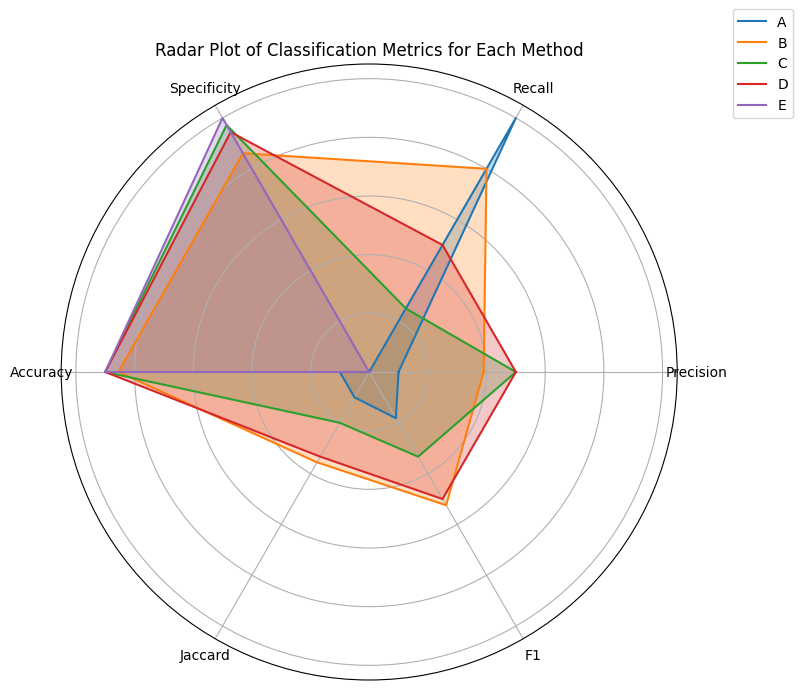
\includegraphics[width=0.5\textwidth]{images/radar_plot.png}
		\caption{The Radar plot}
		\label{fig:radar}
	\end{center}
\end{figure}
  \vspace{-20pt}
 
 \section{Metrics Comparison}
 
 In addition to analyzing all metrics at once, similar to bivariate analysis, we can highlight specific metrics for a more focused evaluation. By plotting methods on a 2-dimensional plane, where the x-axis represents one metric and the y-axis another, we can carefully assess the direct relationships between these values.
 
 \subsection{False Negatives (FN) against False Positives (FP)}
 
 It has already been observed that certain methods yield a high number of false negatives and false positives. Plotting both values on a 2-dimensional plane allows for a more intuitive visualization of which methods are performing better (see the figure \ref{fig:FPyFN}). The closer the methods are to the origin (0,0) — having fewer false positives and false negatives — the more ideal they are.

\begin{figure}[h!]
	\begin{center}  % Usamos el entorno 'center'
		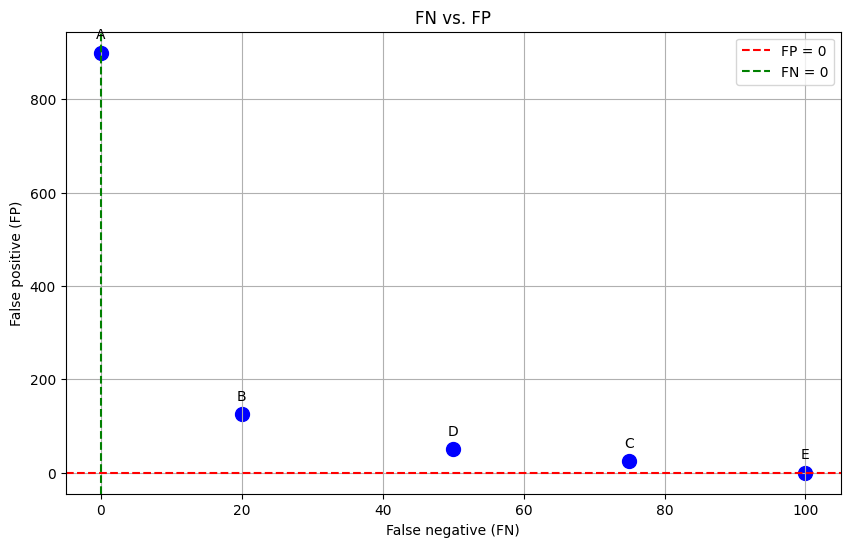
\includegraphics[width=0.49\textwidth]{images/FN_VS_FP.png}
		\caption{FN vs. FP for each method.}
		\label{fig:FPyFN}
	\end{center}
\end{figure}

As it has been a constant in the work methods A and E gave terrible results for the reasons already explained. And the methods B and D stand out positively as expected. 

This visualization is important because false positives (FP) and false negatives (FN) directly impact the overall performance of a classifier. A method that minimizes both types of errors is considered optimal, especially in critical applications like medical diagnosis, where both kinds of mistakes can lead to significant consequences.

\subsection{Precision (PR) against Recall (RC)}

A Precision vs. Recall plot provides insight into the trade-off between these two metrics (see Figure \ref{fig:PRyRC}), improving precision leads to lower recall, and vice versa. This visualization is particularly valuable when dealing with imbalanced classes. By observing the balance between precision and recall, one can determine the optimal threshold that best balances both metrics, allowing for model performance adjustments based on the specific needs of the task.


\begin{figure}[h!]
	\begin{center}
		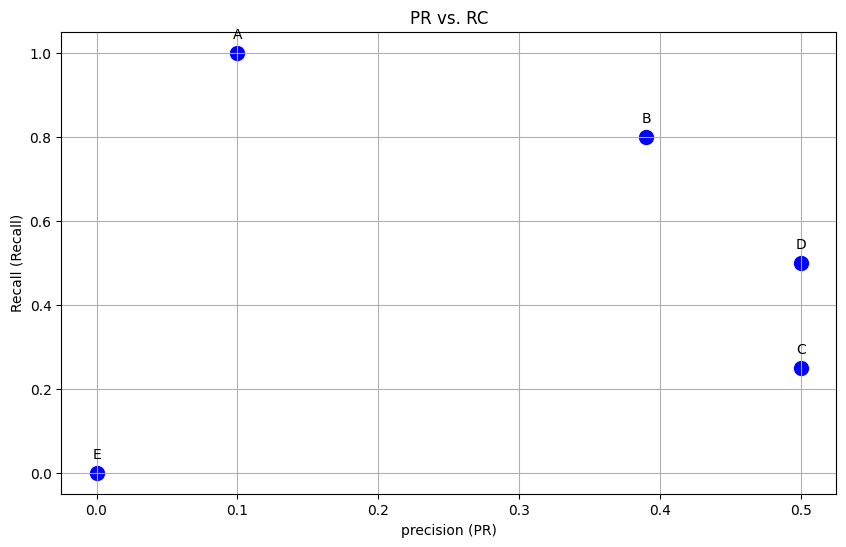
\includegraphics[width=0.6\textwidth]{images/PR_RC.png}
		\caption{PR vs. RC for each method.}
		\label{fig:PRyRC}
	\end{center}
\end{figure}

The most ideal position for a method is close to the point (1,1), indicating high precision and high recall. Method B stands out as the best performing, achieving a balanced high value for both metrics, while method E performs poorly, as expected from previous observations.


\subsection{Accuracy (ACC) vs. F-measure (Fm)}

Analyzing an Accuracy versus F-measure plot allows one to assess how well a classification model performs by considering its overall correctness (accuracy) and its effectiveness in identifying true positives (F-measure). Accuracy, defined as the proportion of correct predictions out of the total predictions, can be a misleading measure in imbalanced datasets where one class is more prevalent, as it tends to inflate the performance of models that prioritize the dominant class. Conversely, F-measure (F1 score) balances precision and recall, reflecting the model’s capability to correctly identify instances of the positive class, which is crucial in cases where the positive class is of particular interest.

By examining the relationship between these two metrics, one can identify models that not only perform well in terms of accuracy but also maintain a good balance in detecting true positives. This type of analysis helps to discern models that offer meaningful and reliable performance, especially in practical applications where the accurate detection of specific classes is critical. As shown in Figure \ref{fig
}, certain methods such as B and D demonstrate both high accuracy and high F-measure, indicating a balanced and effective performance. Meanwhile, Method E, despite its high accuracy, has a relatively low F-measure, suggesting it may be failing to identify positive instances adequately, potentially by overclassifying them as erroneous. This reinforces the importance of F-measure in identifying models that can capture the nuances of the positive class rather than merely achieving high overall accuracy.

\begin{figure}[h!] \begin{center} 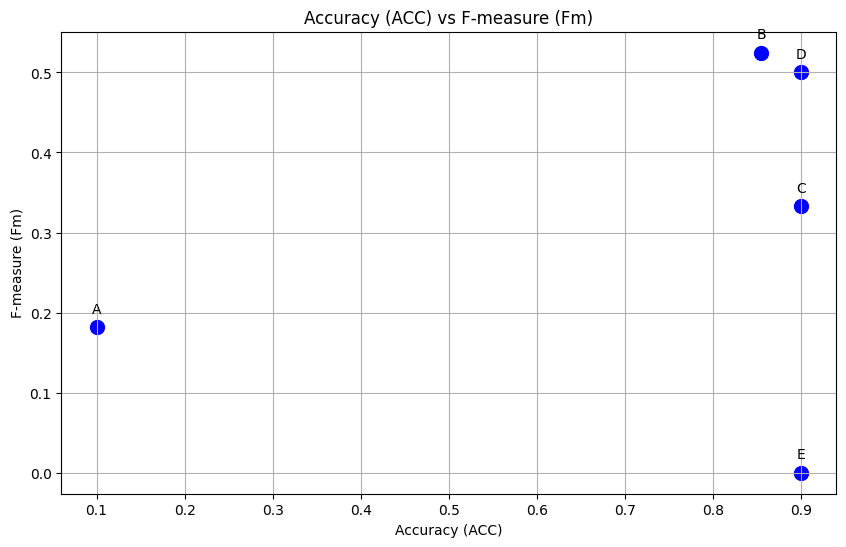
\includegraphics[width=0.6\textwidth]{images/ACC_VS_Fm.png} \caption{ACC vs. Fm for each method.} \label{fig
} \end{center} \end{figure}


\section{Conclusion}
In this study, we compared five classification methods (A, B, C, D, and E) using various performance metrics to assess their effectiveness in handling an imbalanced dataset, particularly for disease prediction. The analysis revealed differences in performance across precision, recall, and F-measure, with Method B standing out as the most balanced.

\begin{itemize}
	\item \textbf{Method B:} This method provides the best overall balance between precision, recall, and F-measure, making it the most robust option for applications that demand both accurate positive identification and high precision.
	
	\item \textbf{Methods A and E:} Both methods show negligible classification capability. Method A predicts only positives, while Method E predicts only negatives, making them ineffective for distinguishing between classes. Their extreme limitations offer no practical value in balanced classification tasks.
	
	\item \textbf{Method C:} This method strikes a moderate balance between precision and specificity. However, its performance is hampered by a significantly high false negative rate, preventing it from reaching the robustness of Method B.
	
	\item \textbf{Method D:} Although this method ranks as the second-best performer, its higher false negative rate compared to Method B reduces its overall effectiveness.
\end{itemize}

\textbf{Method B:} is the most effective classification method for this imbalanced dataset due to its high F-measure and balanced precision and recall. It is recommended for predictive tasks where accurate positive identification and minimizing false positives are critical, even in the context of an imbalanced dataset. Also in a health context, method B is the one that stands out the most because it obtains almost all positive cases, where in disease studies it is very important to maximize the number of true positives.

\section{Repository Github}
Further information, including the source code and full project documentation, can be accessed through the GitHub repository.  \href{https://github.com/Diegodepab/Supervised_Learning_Model_Evaluation_Metrics}{Click here to go to the repository.} 



\bibliographystyle{plain}  % Puedes cambiar "plain" por el estilo de tu preferencia, como apalike, ieeetr, etc.
\bibliography{bibliography}  % Aquí va el nombre de tu archivo .bib (sin la extensión .bib)
\end{document}
